\documentclass{sigchi}

% Load basic packages
\usepackage{balance}  % to better equalize the last page
\usepackage{graphics} % for EPS, load graphicx instead 
\usepackage{mathptmx}
\usepackage[pdftex]{hyperref}
\usepackage{color}
\usepackage{booktabs}
\usepackage{textcomp}
\usepackage{microtype} % Improved Tracking and Kerning
\usepackage{ccicons}  % Cite your images correctly!
\usepackage{multicol}
\usepackage{color} 
\newcommand{\hl}[1]{\colorbox{yellow}{#1}}
\usepackage{xspace}
\usepackage{algorithm} 
\usepackage{algpseudocode} 
\usepackage{booktabs}
\def\algname{SPRING\xspace}


% Paper metadata (use plain text, for PDF inclusion and later
% re-using, if desired).  Use \emtpyauthor when submitting for review
% so you remain anonymous.
\def\plaintitle{A Data-Driven Approach for Inferring Student Proficiency from Game Activity Logs  }
\def\plainauthor{Mohammad H. Falakmasir, Jos\'{e} P. Gonz\'{a}lez-Brenes, Geoffrey J. Gordon, Kristen E. DiCerbo}
\def\emptyauthor{}
\def\plainkeywords{Authors' choice; of terms; separated; by
  semicolons; include commas, within terms only; required.}
\def\plaingeneralterms{Documentation, Standardization}

% llt: Define a global style for URLs, rather that the default one
\makeatletter
\def\url@leostyle{%
  \@ifundefined{selectfont}{
    \def\UrlFont{\sf}
  }{
    \def\UrlFont{\small\bf\ttfamily}
  }}
\makeatother
\urlstyle{leo}

% To make various LaTeX processors do the right thing with page size.
\def\pprw{8.5in}
\def\pprh{11in}
\special{papersize=\pprw,\pprh}
\setlength{\paperwidth}{\pprw}
\setlength{\paperheight}{\pprh}
\setlength{\pdfpagewidth}{\pprw}
\setlength{\pdfpageheight}{\pprh}

% Make sure hyperref comes last of your loaded packages, to give it a
% fighting chance of not being over-written, since its job is to
% redefine many LaTeX commands.
\definecolor{linkColor}{RGB}{6,125,233}
\hypersetup{%
  pdftitle={\plaintitle},
% Use \plainauthor for final version.
%  pdfauthor={\plainauthor},
  pdfauthor={\emptyauthor},
  pdfkeywords={\plainkeywords},
  bookmarksnumbered,
  pdfstartview={FitH},
  colorlinks,
  citecolor=black,
  filecolor=black,
  linkcolor=black,
  urlcolor=linkColor,
  breaklinks=true,
}

% create a shortcut to typeset table headings
% \newcommand\tabhead[1]{\small\textbf{#1}}

% End of preamble. Here it comes the document.
\begin{document}

\title{\plaintitle}

\numberofauthors{4}
\author
{%
  \alignauthor{\mbox{\hspace{-1.85em}Mohammad H. Falakmasir$^{\star, \#} $\;\;\; Jos\'{e} P. Gonz\'{a}lez-Brenes$^\star$ \;\;\; Geoffrey J. Gordon$^\S$ \;\;\; Kristen E. DiCerbo$^\star$}\\
    \affaddr{$^\star$School Research}\\
    \affaddr{Pearson}\\
    \email{\{jose.gonzalez-brenes, kristen.dicerbo\}@pearson.com }\\
    }
  \alignauthor{\vphantom{Mohamamad Jose}
    \affaddr{$^\#$Intelligent Systems Program} \\
    \affaddr{University of Pittsburgh}\\
    \email{falakmasir@pitt.edu}\\
  }
  \alignauthor{\vphantom{Mohamamad Jose}
  	\affaddr{$^\S$Machine Learning}\\
	\affaddr{Carnegie Mellon University} 
  	\email{ggordon@cs.cmu.edu}\\
  }
}

  
\maketitle

\begin{abstract}
Traditional assessments are important in education because they allow collecting evidence about student progress. 
Unfortunately, they can be very tedious to their stakeholders.
In contrast, invisible assessment  unobtrusively gathers  performance data from students' daily activities to make inference about student relevant competency.
We present a novel data analysis pipeline, {Student Profficiency Inferrer from Game data} (\algname), that allows modeling  game playing behavior in educational games.
Unlike prior work, \algname is a fully data-driven method that does not require costly domain knowledge engineering.
We validate our method using data collected from students playing 12 educational mini-games.
Our results suggest that  \algname is accurate to predict Math assessments ($R^2$ =0.55 , Spearman $\rho$=0.82).
%We provide insights in how to use \algname to understand student exploration habits, misconceptions, and how to improve the game design based on their playing strategies.
\end{abstract}

\category{K.3.1}{Computer Uses in Education.}
{}
\keywords{Educational Games, Student Modeling, Stealth Assessment}

\section{Introduction}
Educational assessments are important because they collect evidence about about  whether  the teaching goals are being met.
Unfortunately, the process of  administering assessments is usually disconnected to the learning environment, and  it is often  disruptive to the classroom. 
In many developed countries, students now find themselves spending increasing amounts of time preparing and taking tests instead of learning~\cite{hofman2015rebalancing}.
For example, a  survey of the current state of testing in America revealed that students are taking an average of 113 standardized tests between pre-K and highschool~\cite{lazarin2014testing}.  %http://www.npr.org/sections/ed/2014/11/17/362339421/testing-how-much-is-too-much 
For these reasons, it is not surprising that the recent political climate and the general population have been weighing in on the question of whether students are being tested too much~\cite{lazarin2014testing}.


According to Evidence Centered Design (ECD)~\cite{mislevy2012design}, the goal of assessment is to characterize the strength of evidence regarding claims one wants to make about individuals or groups.
Therefore, the assessment process involves identifying, organizing, or creating activities for students so we may observe that evidence.
An interesting alternative to traditional (summative) assessment is invisible (often called stealth) assessment~\cite{shute2013stealth},
where the evidence is gathered from leaners unobtrusively from the digital interactions of their ongoing activities.
This data is used  to understand claims regarding what students know and what they can do \cite{shute2009melding}.
Stealth assessment is also intended to reduce or eliminate test anxiety, while not sacrificing validity and reliability \cite{shute2008you}.

% I generate tables with:  http://www.tablesgenerator.com/

A promising opportunity for invisible assessment is using log data collected from educational games.
Unfortunately, engineering a system that parses logs is costly and time-consuming.
For example, prior work~\cite{shute2013stealth, shute2009melding} has relied extensively on subject matter expertise to define a student model in form of a  Bayesian Network to build both the competency model, and to extract features of the performance data.
%\hl{confirm if it's regression}
%\hl{give examples of the things they did manually}.

Our motivation is that invisible assessment from game data may become more accurate and cheaper to implement if the domain knowledge engineering could be automated by a data-driven process.
Game data is often logged  with what we call a \textit{slot and filler} structure.
In Table~\ref{tbl:log_example}, we show a simplified example of a real educational game log that uses slot and filler structure.
The slots are discrete sets of events that are initiated by the leaner.
Each slot may accept zero to multiple fillers. 
Each filler represents a value of a property of the slot event.
For example, a ``move" event  that represents that the learner moved an object in the screen may have an $x$ and $y$ fillers, to represent the target position in two-dimensional space.


\begin{table}[tbh]
\caption{An example fragment of a log from an educational game. \label{tbl:log_example}}
\begin{tabular}{@{}llll@{}}
\toprule
\textbf{Id}             & \textbf{User Id} & \textbf{Event Name} & \textbf{Event Data}        \\ \midrule
1                       & ABC              & Game Start          & \{ \}                        \\
2                       & ABC              & Move Object         & \{endPosX:363,endPosY:82\} \\
3                       & ABC              & Move Object         & \{endPosX:361,endPosY:54\} \\
4                       & ABC              & Insert Ruler        & \{EndOffsetX: -14\}        \\
\multicolumn{1}{c}{...} &                  &                     &                            \\ \bottomrule
\end{tabular}
\end{table}
% http://www.tablesgenerator.com/#


Unfortunately, conventional machine learning algorithms cannot input slot and filler data, as they  work in  structures called \textit{feature vectors} or \textit{sequences}.
Prior work~\cite{sequences} provides a   review of  the difference between feature vectors and sequences.
A feature vector representation requires mapping an observation onto a fixed number of features.
It is not trivial to map sequences of student actions that can be of arbitrary length into a feature vector that needs to be of a predetermined lenth.
Traditional feature vector classifiers,  like logistic regression or decision trees,  that are used in off-the-shelf data mining packages, such as Weka \cite{hall2009weka}, cannot  use slot and filler data. 
In contrast, machine learning algorithm that allow sequential representations, like Hidden Markov Models (HMM), require a parametric model with the same number of dimensions for every observation, which does not occur in slot and filler structures.



In this paper, we propose \textit{Student PRofficiency INferrer from Game data} (SPRING), a novel data analysis pipeline that models game playing behavior.
\algname allows modeling raw data in slot and filler structure.
We demonstrate our approach on real student game playing data.
Our experiments suggest that \algname can be used to predict student proficiency  without costly domain expertise.


%Our framework is designed in a way that can capture sequential decision making process of students in a way that is representative of their mastery with minimum reliance on expert knowledge specific to the skill domain.

%However, the unrestricted nature of educational games allows students to explore and interact with a learning environment in a broader more meaningful way and even the student logs from educational games that are designed based on the ECD framework usually involves observations that are not directly linked to the main educational objectives. 
%Moreover, off-the-shelf probabilistic models and machine learning methods are unable to handle data collected from game logs because of the objective nature of the observations throughout the evidence identification and accumulation process of the ECD framework \cite{dicerbo2012implications}. 

%We faced three main challenges in this process. The majority of student interactions with our educational game involve moving objects (tiles) into pre-defined locations in the game level interface. Our first challenge was to combine these movements with continuous distribution with other interactions that are less frequent and have discrete distribution. Our second challenge was to find pattern that are predictive of student mastery. A large portion of student interactions are based on the logic of the games and we would like a method with minimal human authoring that is capable of inferring patterns that are able to distinguish between high- and low-performing students in each game level. Our educational game has 12 game levels in a predesigned order and students cannot progress to the next game level unless they successfully finish the previous game level. Early game levels involve basic concepts and the complexity and number of skills required to complete task increases by progressing through game levels. Our last challenge was to find a way to aggregate the patterns extracted from multiple game levels in an ensemble method that predicts the post-test scores.


\section{SPRING Framework}
Algorithm~\ref{alg:spring} describes the SPRING algorithm.
\hl{Describe in words}
We now describe  the discretization, sequence modeling and regression steps.  
\hl{Why only these steps?}

\hl{This algorithm needs to be rewritten to be pseudo-code, or in an illustration}.
\hl{ Right now it's not understandable, for example, we never talk about post-tests}
\hl{We need to explain the input and output.}
\hl{I agree a  picture may be more suitable, but \textit{every} step has to be explained}

\begin{algorithm}
\begin{algorithmic}
\State Extract Clusters from 2D movements (x, y) \hl{why only of moves? it's about fillers}
\State Use Cluster IDs to transform movements into multinomial variables  \hl{What are cluster IDs? what are multinomial variables?}
\State Use Converted Trajectories to Learn the State Sequence for High- and Low-Performing Students \hl{What are converted trajectories? Where do they come from?}
\State Calculate the likelihood of Student Trajectories in the Held-Out Set 
\State Train a Linear Regression Model using Student Trajectories on the Development Set
\State Predict Student Post-Test Scores \h
\end{algorithmic}
\caption{The \algname pipeline. \label{alg:spring}}
\end{algorithm}
% I am not sure if we need a algorithm. A picture might be more suitable.





\subsection{Discretization}
In order to gather the evidence for learning from student trajectories \hl{?} of interactions with the game, we needed to create features that are homogenous \hl{?} and can be used in an interpretable model. 
Each student trajectory consists of a sequence of discrete actions accompanied by some details that are usually continuous variables. 
Our main challenge in this phase was to transform the movements into a set of observable values that are usefull as evidence for learning.
In order to make sure that the model is generalizable across multiple game levels, we first used DBSCAN \hl{Say that in our implementation we used DBSCan, but the algorithm allows any clustering} clustering algorithm \cite{ester1996density} on the $x$ and $y$ coordinates of the movements to extract the crucial regions within the game interface. 
DBSCAN was a good candidate because it can find arbitrarily shaped clusters and does not require one to specify the number of clusters in the data a-priori. 
It is also robust to outliers which in our case can be interpreted as noisy movements that are not representative of learning competency. 
After clustering, we transformed each movement into its cluster number and considered outliers as a separate cluster. 
Figure~\ref{fig:figurecluster} shows the clusters detected for one of the game levels.

\begin{figure}
	\centering
	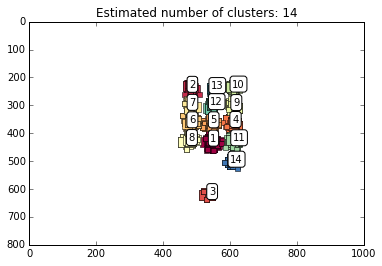
\includegraphics[width=0.9\columnwidth]{figures/cluster}
	\caption{The clusters detected for game level 11, \textit {You Kraken Me Up!}, using DBSCAN method. We transform each movement action into corresponding cluster number during the discretization step.}~\label{fig:figurecluster}
\end{figure}


\subsection{Sequence Modeling}
In the modeling phase, we hypothesized that high- and low-performing students have similar usage patterns that are representative of their sequential decision-making process. 
Our model should be able to successfully capture this difference across different game levels and use it to predict post-test scores.
Hidden Markov Models are good candidate for the task of unsupervised analysis of sequential data.
Given the sequence of student actions, we aim to infer meaningful sequence of (latent) states, which describe the process that generated the actions, along with statistical patterns that can describe and distinguish those states.
Since a large portion of student interactions are based on the logic of the game, we had no idea about the number of states and what they mean.
As a result, we used the Hierarchical Diriclet Process HMM (HDP-HMM) \cite{fox2008hdp}, which is allows state spaces of unknown size to be learned from data. 
HDP-HMM defines a \textit{hierarchical Dirichlet process} prior on transition matrices over countably infinite state spaces and is able to make a principled choice of how many states it needs based on the complexity of its training data. 
For details on training methods please refer to \cite{fox2008hdp}.

We used the output of the discretization step as sequence of multinomial observations and trained two HDP-HMMs, one for high-performing and the other for low-performing students using the student trajectories in our development set. After that, we calculated the likelihood of student trajectories in the heldout set using each of the HMMs and used the likelihood difference as a feature in a regression model for predicting the post-test scores.

\subsection{Regression}

In this phase, we created a linear regression model using 5-fold cross-validation \hl{So spring requires 5fold cross validation for it to work? ;-)} on the data in our development set. We tried different regularization methods (lasso and ridge regression) to find the optimum parameters and tested it on the heldout set in order to evaluate our model. 
\hl{What are the features? Write equation}

\section{Empirical Evaluation}

\subsection{Game Environment}
\textit {Alice in AreaLand} is an educational game developed for research purposes. It focuses on teaching and assessing geometric measurement, specifically the understanding of area, among 6th grade students. The game targets three main stages in the development of area: 1) area unit iteration, 2) use of unit squares to measure area, and 3) use of composites to measure area. The current version has 12 game levels. A simple student scenario involves covering a 2D area with smaller unit squares placed end-to-end in non-overlapping fashion, combining the single squares into rows or columns, and then determining the number of rows or columns needed. Figure~\ref{fig:figurekracken} shows a screenshot of one game level.

\begin{figure}
	\centering
	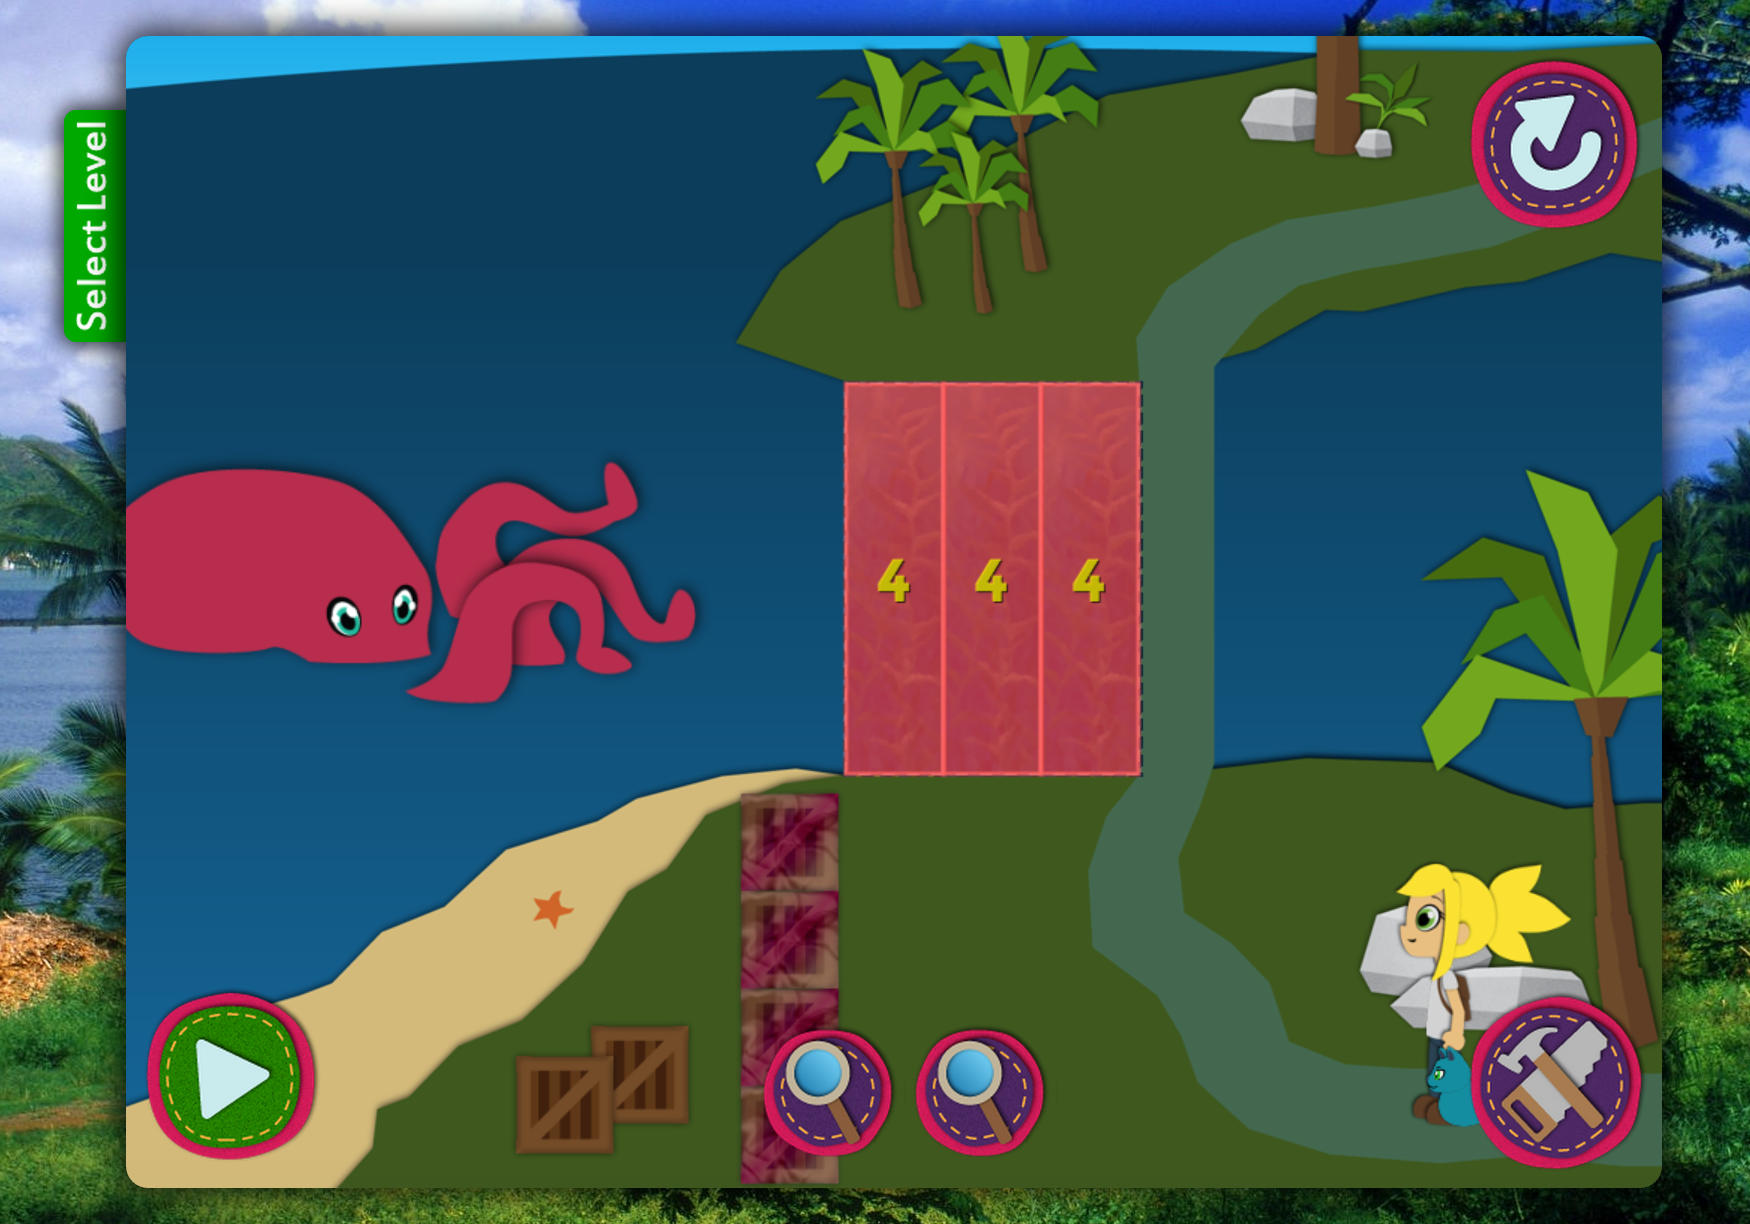
\includegraphics[width=0.9\columnwidth]{figures/kracken}
	\caption{A screenshot of hint provided in game level 11, \textit {You Kraken Me Up!}, in \textit {Alice in AreaLand}. Students should combine four squares into a column and create three copies of the column to cover the designated area and prevent the octopus from attacking \textit {Alice} while she crosses the bridge.}~\label{fig:figurekracken}
\end{figure}

Throughout the game,  \textit {Alice} is accompanied by \textit {Flat Cat} -- an assistant character who provides feedback and scaffolding to the player in the beginning of each game level and upon request when students push a hint button (represented by two magnifiers at the bottom center of Figure ~\ref{fig:figure1}). Earlier game levels are designed for students to learn about area unit iteration and usually require them to cover a number of predefined areas with unit squares (not necessarily in a non-overlapping fashion). By advancing through game levels, students are presented with three tools: \textit {Gluumi} for combining unit squares by gluing them together; \textit {Multy}, for making copies of different objects; and \textit {Esploda} for breaking compound shapes into single units.  There is no limit for completing a game level regarding time or number of actions students may execute. The students press the \textit {Go Alice} button (bottom left corner of Figure~\ref{fig:figure1}) if they deem their performance to be satisfactory for \textit {Alice} to proceed. Based on the covered area and the arrangement of the tiles, they either advance to the next level or receive a feedback and stay in the same level.

\subsection{Dataset} 
Our dataset consists of time-stamped interactions of 129 students in 12 game levels. 
For 77 students, we also have post-test scores from a paper-based exam with 20 questions in the 3 skills of geometric measurement.
In total, there are 88,458 events recorded in the dataset from 1,510 game sessions, meaning that student tried some of the game levels for multiple times.
Based on the ECD framework, beginning levels only involve area unit iteration skill and the other skills and related features are gradually added to the later game levels.
We only used the trajectories of the students who participated in the post-test.
In the case of multiple attempts in a game level, we only considered the trajectory from the first attempt.

\hl{histogram of events}
\hl{descriptive statistics} 

\subsection{Experimental Setup}
First we divide students into two groups, one (\%80) for training and development purposes and the other (\%20) for test and verification.
In the synthesis phase, we transform log data of different nature (eg. movements, use of the tools, requests for hints) in each game level to observable values that can be used as evidence for learning.
In the modeling phase, we use the observations to train two Hidden Markov Model (HMM)s that capture the sequence of actions for high- and low-performing students.
In the aggregation phase, we uses the likelihood of students' sequence of action in order to build a regression model that is predictive of the post-test results.
Finally, we test the regression model on the held-out set (\%20) and report the results.


\subsection{Results}
In order to evaluate our regression model we decided to compare its performance agains two baselines: 1) A regression model that uses success and failure of students in each game level as feature \hl{Write equation}and 2) A regression model that uses the sequence lengths in each game level \hl{Write equation}. 
Our model was able to significantly outperform both baselines regarding to mean absolute error and root mean squared error. 
Moreover, the $R^2$ correlation and Spearman $\rho$ of our predicted values with the true values was much higher than both baselines. Table \ref{tab:results} shows the results.


\begin{table}[tbh]
	\centering
	\caption{The results of predicting post-test scores using three different feature sets}
	\label{results}
	\begin{tabular}{@{}lllll@{}}
		\toprule
		\begin{tabular}[c]{@{}l@{}}Prediction\\ Method\end{tabular}            & \begin{tabular}[c]{@{}l@{}}$R^2$\end{tabular} & \begin{tabular}[c]{@{}l@{}}$\rho$\end{tabular} & \begin{tabular}[c]{@{}l@{}}MAE \end{tabular} & RMSE \\ \midrule
		\begin{tabular}[c]{@{}l@{}}Sequence Length\\ (Normalized)\end{tabular} & 0.06                                                     & 0.79                                                 & 3.24                                                          & 4.15 \\
		Success / Failure                                                      & 0.01                                                     & 0.63                                                 & 3.22                                                          & 4.14 \\
		\algname                                                       & 0.55                                                     & 0.82                                                 & 2.84                                                          & 3.35 \\ \bottomrule
	\end{tabular}
\end{table}

\hl{Show residual plot}
\hl{Show confidence intervals}

\section{Relation to Prior Work}
In order to deal with such highly unstructured data, researchers often use carefully designed network structures (such as Bayesian Networks \cite{albrecht1998bayesian}) or game-specific heuristics and benchmarks generated by experts playing the game \cite{mandel2014offline,tastan2011learning}. However, this approach is extremely labor intensive and might fail to capture meaningful patterns in student exploratory habits within the game. Given these limitations, data-driven analysis of student interactions provides a powerful alternative that facilitates the discussions around what does and does not work in a particular educational game.

The potential of computer games for educational purposes has been of interest since nearly the beginning of videogames. Unlike video games, which focus on creating an entertaining experience for the user, educational games require principles and strategies that engage students while maximizing their learning gain. Therefore, data-driven analysis of student behavior is crucial to better understand the learning process and improve the tools in the future.

There have been numerous attempts among the educational research community to develop analytic methods and build predictive models based on the data from educational games. \textit {Rumble Blocks}  is an educational game designed to teach basic concepts of structural stability and balance to children in grades K-3 (ages 5-8 years old). Harpstead et al. \cite{harpstead2014using}, studied the alignment of game to its target learning goals by examining whether student solutions follows the targeted principals. They employ clustering techniques on the individual solutions created by actual students and use principle-relevant metric (PRM) to measure how closely the representative solution embodies a specific targeted principle. The results demonstrated a misalignment between the feedback provided to students and the targeted knowledge.

\textit {Battleship Numberline} is another educational game for understanding fraction using number line estimation. Students attempt to explode target ships and submarines by estimating numbers on a number line. Lomas et al. \cite{lomas2013optimizing} performed a large-scale online experiment in order to study the effect of challenge on player motivation and learning. They presented different configurations of the game for different groups of students and used a combination of time spent and challenges attempted as a measure of engagement and the average success rate of each design configuration as a measure of challenge. The results showed a linear correlation between challenge (difficulty) and engagement, meaning the easier the game, the longer students played.

\textit {Refraction} is another educational game for learning about fractions by splitting laser beams into fractional amounts to target spaceships by avoiding asteroids. Liu et al. \cite{liu2013predicting}, created an ensemble algorithm that combines elements of Markov models, player heuristic search, and collaborative filtering techniques with state-space clustering in order to predict player movements on last game-level based on the history of movements in previous game levels. Lee et al. \cite{lee2014learning} extended the former framework by building state-action graph and using feature selection techniques to reduce the number of features for each state. To ensure extensibility, they also tested the framework on another game \textit {DragonBox} and reported improvement over a Markov predictor.

\section{Conclusion}
\hl{Limitation, we don't compare to Valerie Schultz}

\hl{Limitation, we don't control for game ability like Valrerie does}

\hl{Limitation, we only used data from Alice in wonderland}

\hl{Method is accurate}


\bibliographystyle{SIGCHI-Reference-Format}
\bibliography{references}

\end{document}
